%!TeX root=main.tex
\chapter{آزمایش‌ها و نتیجه‌ها}
\thispagestyle{empty}

تمامی کد‌های پروژه در 
\href{https://github.com/yegmor/Final_Project}{این لینک}
تحت لیسانس 
\href{https://choosealicense.com/licenses/mit/}{\lr{MIT}}
قابل دسترس است.
لازم به ذکر است که نمودار‌ها در پوشه
\textbf{\lr{results}}
و مدل‌های آموزش دیده در پوشه
\textbf{\lr{models}}
قرار داده شده‌اند.

\section{مشخصات محیط اجرای کد}
\subsection{سخت افزار و سیستم عامل}
\lr{GPU.1080Ti.xlarge}
با رم 
\lr{31.3 GB}
که دارای ۶ 
\lr{vCPU (virtual CPU)}
است و سیستم عامل 
\lr{Ubuntu 18.04}
استفاده شده است.

\subsection{نرم‌افزار و کتاب‌خانه}
کد‌ها به زبان 
\lr{Python}
و با استفاده از چارچوب
\LTRfootnote{Framework} \lr{PyTorch}
نوشته شده‌اند.
\\
برای اجرا کدها از سخت‌افزار
با دستور 
\lr{nvidia-smi}
میزان استفاده از 
\lr{GPU}
را مشاهده نمود. 
\\
تمامی کتاب‌خانه‌ها و پکیج‌های استفاده شده به همراه ورژن آن ها در فایل 
\lr{requirements.txt}
آورده شده است. برای نصب پکیج‌های مورد نیاز برای اجرا کد، می‌توان از دستور زیر استفاده کرد:
\begin{latin}
	\pythonline{pip install -r requirements.txt}
\end{latin}

\section{مجموعه داده}
در این پروژه از مجموعه‌ داده MNIST استفاده می‌کنیم که این مجموعه‌ داده مشتمل بر ۶۰۰۰۰ عکس ۲۸*۲۸ پیکسلی برای آموزش شبکه و ۱۰۰۰۰ عکس
\lr{۲۸*۲۸}
پیکسلی برای تست شبکه است.

\section{بخش‌های کد و نحوه‌ اجرایشان}
کدهای پروژه در سه بخش زیر قابل اجرا هستند:
\subsection{آموزش شبکه هدف}
در این بخش، پس از بارگیری مجموعه داده های تست و آموزش، مدل هدف آموزش می‌بیند و سپس مدل آموزش دیده ذخیره می‌شود و نمودارهای مربوط به عملکرد شبکه در طول آموزش نیز رسم می‌شود. در آخرین بخش عملکرد شبکه بر روی مدل آموزش دیده نهایی اعلام می‌گردد.
\begin{latin}
	\pythonline{python3 train\_target\_model.py}
\end{latin}

\subsection{آموزش شبکه
\lr{Adv-GAN}}
در این بخش، پس از بارگیری مجموعه داده‌های تست و آموزش و مدل هدف از پیش آموزش دیده شده‌، مدل 
\lr{Adv-GAN}
آموزش می‌بیند و در همین حین ضرر‌های هر بخش از مدل نیز اعلام می‌شود. سپس مدل آموزش دیده ذخیره می‌شود و نمودارهای مربوط به عملکرد شبکه در طول آموزش نیز رسم می‌شود.
\begin{latin}
	\pythonline{python3 train\_advGAN\_model.py}
\end{latin}

\subsection{ارزیابی نمونه‌های تقابلی تولید شده}
در این بخش، مجموعه داده‌های تست و آموزش، ورژن نهایی مدل هدف و قسمت مولد 
\lr{Adv-GAN}
آموزش دیده شده بارگیری می‌شوند و سپس با تولید نمونه‌های تقابلی و تست کردن آن‌ها بر روی مدل هدف، عملکرد شبکه با رسم ماتریس درهم‌ریختگی
\LTRfootnote{Confusion Matrix}
و اعلام دقت 
\LTRfootnote{Accuracy}
و امتیاز اف-۱ 
\LTRfootnote{F1-Score}
نشان داده می‌شود.
\begin{latin}
	\pythonline{python3 test\_adversarial\_examples.py}
\end{latin}

\section{معماری و تنظیمات شبکه‌های عصبی}
\subsection{مدل هدف}
در شکل 
\ref{target_model_arch}
معماری شبکه هدف به عنوان دسته‌بند مجموعه‌ داده MNIST آورده شده است. همچنین تنظیمات پارامترهای آموزش شبکه به صورت زیر است:
\begin{itemize}
	\item \lr{Epoch}: 40 
	\item \lr{Batch Size}: 256 
\end{itemize} 
\begin{figure}[H]
	\center{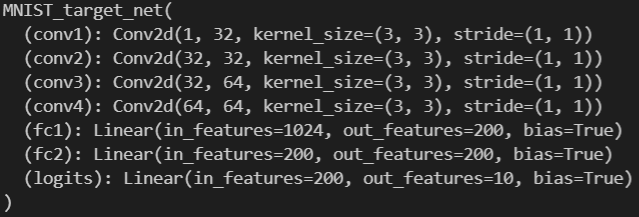
\includegraphics[width=\linewidth]{images/target_model_arch.png}}
	\caption{معماری شبکه هدف}
	\label{target_model_arch}
\end{figure}


\subsection{مدل 
\lr{Adv-GAN}}
تنظیمات پارامترهای آموزش شبکه به صورت زیر است:
\begin{itemize}
	\item \lr{Epoch}: 60 
	\item \lr{Batch Size}: 128 
\end{itemize}

\subsubsection{شبکه مولد}
این شبکه دارای سه بخش است که به ترتیب در ادامه‌ی هم قرار دارند:
\begin{enumerate}
	\item
	کدگزار
	\LTRfootnote{Encoder}
	\begin{figure}[H]
		\center{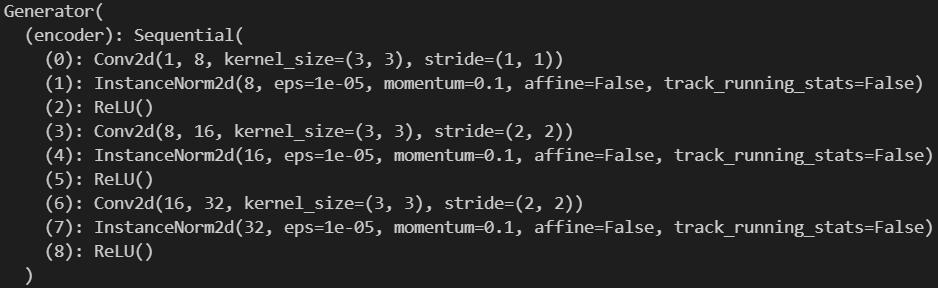
\includegraphics[width=\linewidth]{images/gen_arch_enc.png}}
		\caption{معماری بخش‌ کدگزار شبکه مولد}
		\label{gen_arch_enc}
	\end{figure}

	\item
	گلوگاه
	\LTRfootnote{Bottleneck}:
	این بخش متشکل از ۴ بلوک Resnet یکسان می‌باشد که معماری اولین بلوک آن در شکل 
	\ref{gen_arch_bottleneck}
	آورده شده است.
	\begin{figure}[H]
		\center{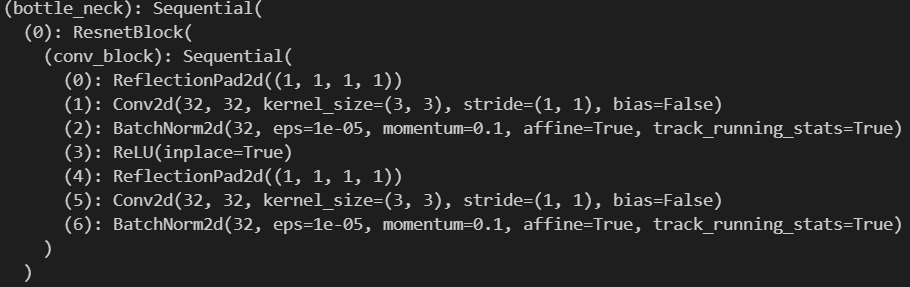
\includegraphics[width=\linewidth]{images/gen_arch_bottleneck.png}}
		\caption{معماری یک بلوک
			\lr{Resnet}
			در بخش گلوگاه شبکه مولد}
		\label{gen_arch_bottleneck}
	\end{figure}

	\item
	کدگشا
	\LTRfootnote{Decoder}
	\begin{figure}[H]
		\center{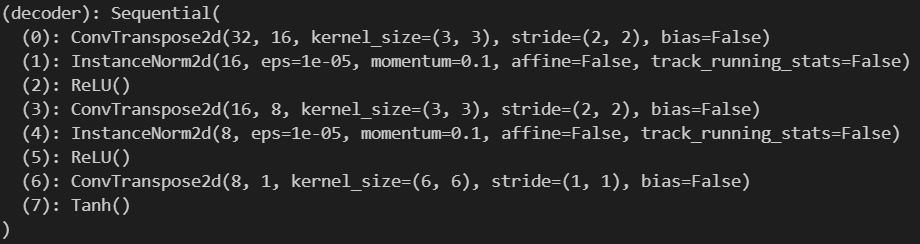
\includegraphics[width=\linewidth]{images/gen_arch_dec.png}}
		\caption{معماری بخش کدگشا شبکه مولد}
		\label{gen_arch_dec}
	\end{figure}
\end{enumerate}

\subsubsection{شبکه تمییز‌دهنده}
\begin{figure}[H]
	\center{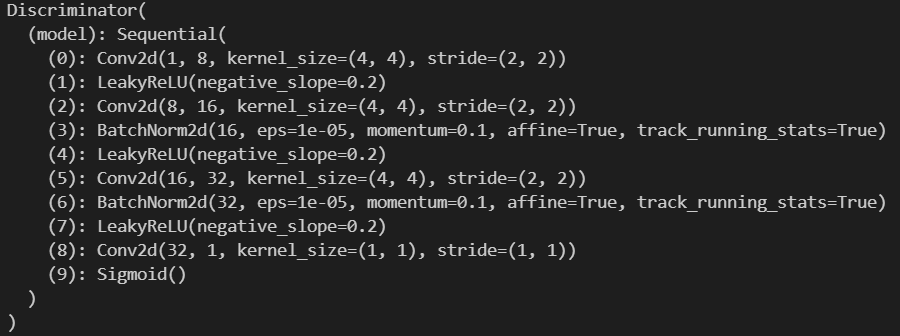
\includegraphics[width=\linewidth]{images/desc_arch.png}}
	\caption{معماری شبکه تمییزدهنده}
	\label{desc_arch}
\end{figure}

\newpage
\section{نتایج عملکرد شبکه هدف قبل از حمله}
در شکل 
\ref{before_targeted_model_accuracy}
نمودار عملکرد دقت شبکه در طول آموزش شبکه هدف بر روی داده تست و آموزش آورده شده است و همان طور که مشاهده می‌شود دقت نمونه با افزایش تعداد دورهای آموزش بهتر می‌شود.
\begin{figure}[H]
	\center{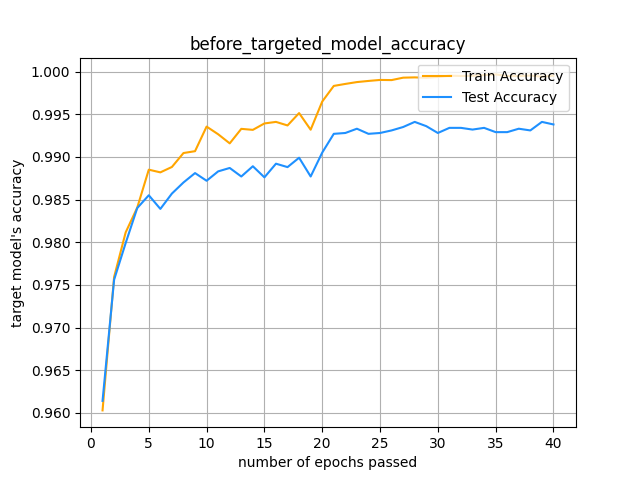
\includegraphics[width=\linewidth]{images/before_targeted_model_accuracy.png}}
	\caption{نمودار دقت شبکه هدف قبل از حمله}
	\label{before_targeted_model_accuracy}
\end{figure}
 به همین منوال در شکل 
\ref{before_targeted_model_loss}
مشاهده می‌شود که ضرر شبکه بر روی هر دو نوع مجموعه داده نزولی است.
\begin{figure}[H]
	\center{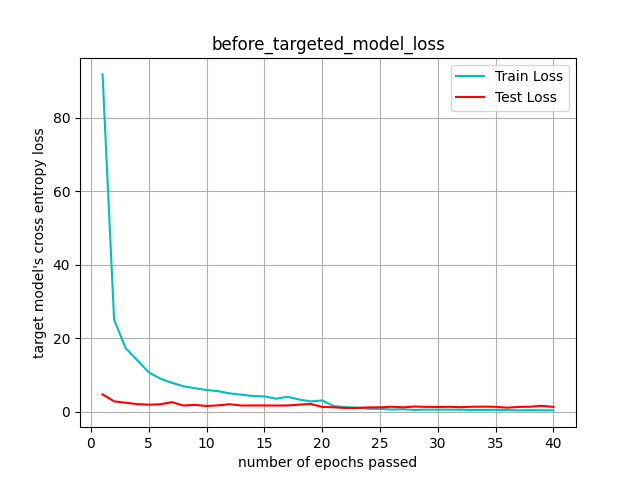
\includegraphics[width=\linewidth]{images/before_targeted_model_loss.png}}
	\caption{نمودار ضرر شبکه هدف قبل از حمله}
	\label{before_targeted_model_loss}
\end{figure}

در نهایت، پس از پایان آموزش شبکه هدف، نتایج عملکرد شبکه بر روی مجموعه داده تست مطابق شکل 
\ref{testset_statistics_before}
است و می‌توان گفت که شبکه از ۱۰۰۰۰ نمونه تست تنها ۷۰ مورد را به درستی دسته‌بندی نکرده است و ۹۹۳۰ مورد را کاملا درست تشخیص داده است.
\begin{figure}[H]
	\center{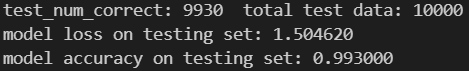
\includegraphics[width=\linewidth]{images/testset_statistics_before.png}}
	\caption{عملکرد شبکه هدف بر روی داده
		 \textbf{تست}
		  قبل از حمله}
	\label{testset_statistics_before}
\end{figure}

\newpage
\section{آموزش شبکه
\lr{Adv-GAN}}
در شکل 
\ref{discriminator_generator_GAN_model_performance}
نمودار ضرر برای مولد و تمییزدهنده شبکه 
\lr{Adv-GAN}
آورده شده است. همان طور که انتظار می‌رود هر چه تعداد دورهای بیشتری شبکه آموزش می‌بیند، مولد در تولید نمونه‌های طبیعی‌تر (ضرر نزدیک به ۱) بهتر می‌شود و همین‌طور تمییزدهنده در تشخیص نمونه تقلبی و تولید شده از نمونه‌ اصلی و طبیعی (ضرر نزدیک به ۰) عملکرد بهتری پیدا می‌کند.
\begin{figure}[H]
	\center{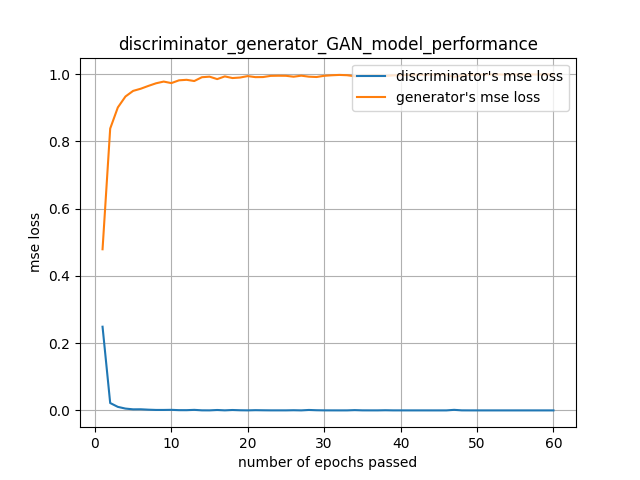
\includegraphics[width=\linewidth]{images/discriminator_generator_GAN_model_performance.png}}
	\caption{نمودار ضرر مولد و تمییز دهنده شبکه
	\lr{Adv-GAN}}
	\label{discriminator_generator_GAN_model_performance}
\end{figure}

\newpage
در شکل 
\ref{perturbation_GAN_model_performance}
نمودار ضرر دستکاری‌ای که برای تولید نمونه‌ تقابلی بر روی تصویر اصلی اعمال می‌شود آورده شده است. طبق انتظار، هر چه تعداد دورهای بیشتری شبکه آموزش می‌بیند، شبکه 
\lr{Adv-GAN}
نمونه‌های تقابلی با دستکاری کمتری می‌سازد و لذا نمونه‌های تولیدی به نمونه‌های طبیعی‌ نزدیک تر و مشابه تر (ضرر نزدیک به ۰) هستند.
\begin{figure}[H]
	\center{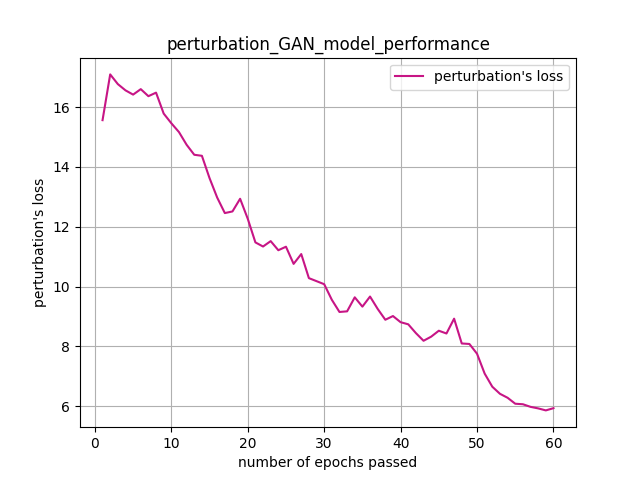
\includegraphics[width=\linewidth]{images/perturbation_GAN_model_performance.png}}
	\caption{نمودار ضرر دستکاری شبکه
		\lr{Adv-GAN}}
	\label{perturbation_GAN_model_performance}
\end{figure}

\newpage
در شکل 
\ref{adversarial_GAN_model_performance}
نمودار ضرر تقابلی‌ که کمینه کردن آن هدف اصلی شبکه است آورده شده است. مشاهده می‌شود با بیشتر شدن تعداد‌ دورهایی که شبکه آموزش دیده است، نمونه‌های تقابلی بیشتر و بیشتر می‌توانند شبکه را فریب بدهند و در دسته‌بندی متفاوت از دسته‌ی تصویر اصلی قرار بگیرند. این ضرر در اصل، عملکرد شبکه
\lr{Adv-GAN}
در گول زدن شبکه هدف را نشان می‌دهد و هر چه این ضرر به ۰ نزدیک‌تر باشد به این معنی است که که شبکه هدف در مقابل حمله ضعیف‌تر و ضعیف‌تر می‌شود.
\begin{figure}[H]
	\center{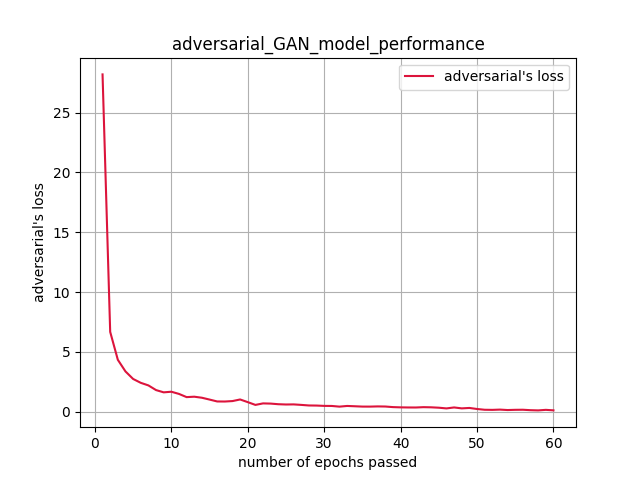
\includegraphics[width=\linewidth]{images/adversarial_GAN_model_performance.png}}
	\caption{نمودار ضرر تقابلی شبکه
		\lr{Adv-GAN}}
	\label{adversarial_GAN_model_performance}
\end{figure}

\newpage
در شکل
\ref{adversarial_GAN_model_performance}
نموداری از هر ۴ ضرر شبکه‌
\lr{Adv-GAN}
به صورت یکجا آورده شده است.
\begin{figure}[H]
	\center{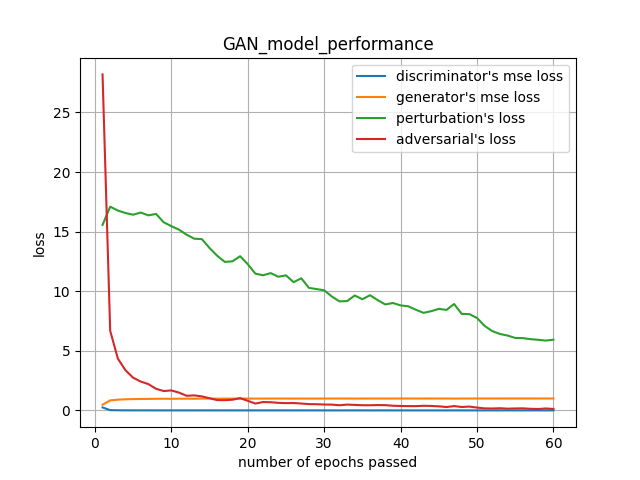
\includegraphics[width=\linewidth]{images/GAN_model_performance.png}}
	\caption{نمودار همه ضررهای شبکه
		\lr{Adv-GAN}}
	\label{GAN_model_performance}
\end{figure}

\newpage
\section{نتایج عملکرد شبکه هدف پس از حمله}
پس از اینکه شبکه 
\lr{Adv-GAN}
آموزش دیده شد و نمونه‌های تقابلی تولید شده توسط بخش مولد این شبکه را به مدل هدف داده شد، نتایج عملکرد شبکه هدف بر روی مجموعه داده آموزش در شکل 
\ref{trainset_statistics}
و مجموعه داده تست در شکل 
\ref{testset_statistics}
آورده شده است.
\begin{figure}[H]
	\center{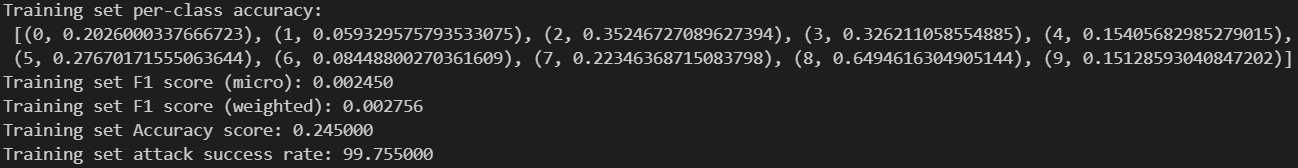
\includegraphics[width=\linewidth]{images/trainset_statistics.png}}
	\caption{عملکرد شبکه هدف بر روی داده
		 \textbf{آموزش}
		  پس از حمله}
	\label{trainset_statistics}
\end{figure}
\begin{figure}[H]
	\center{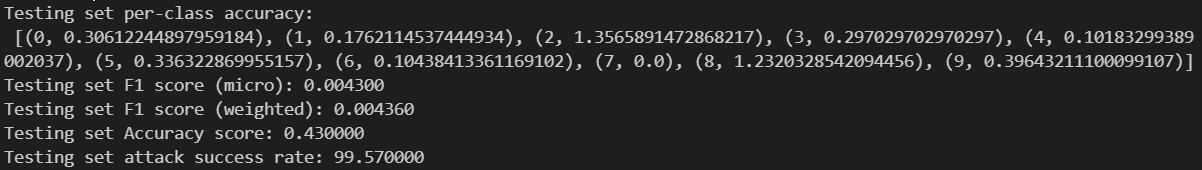
\includegraphics[width=\linewidth]{images/testset_statistics.png}}
	\caption{عملکرد شبکه هدف بر روی داده
		 \textbf{تست}
		  پس از حمله}
	\label{testset_statistics}
\end{figure}
همان‌طور که مشاهده می‌شود در هر دو مجموعه داده تست و آموزش میزان موفقیت حمله بالاتر از
\lr{۹۹/۵٪}
است و یعنی شبکه‌ هدف که تا قبل از این حمله تنها ۷۰ مورد از مجموعه داده تست را به درستی تشخیص نمی‌داد، الان تنها حدود ۴۳ مورد را به درستی دسته‌بندی می‌کند.
\newpage
\section{نمونه‌های تقابلی و مدل هدف}
پس از اینکه شبکه 
\lr{Adv-GAN}
آموزش دیده شد، تنها شبکه مولد را بارگیری کرده و سپس با دادن یک نویز تصادفی نمونه‌ تقابلی تولید می‌شود.
\\
در شکل 
\ref{trainset_imgs_matrix} 
و 
\ref{testset_imgs_matrix} 
برای حالت‌های مختلف برچسب اصلی و پیش‌بینی شده، نمونه‌های تقابلی آورده شده‌اند. در این دو شکل، ردیف‌ها نشان دهنده برچسب و کلاس اصلی و ستون‌ها نشان‌دهنده برچسب پیش‌بینی شده توسط مدل هدف هستند.
\begin{figure}[H]
	\center{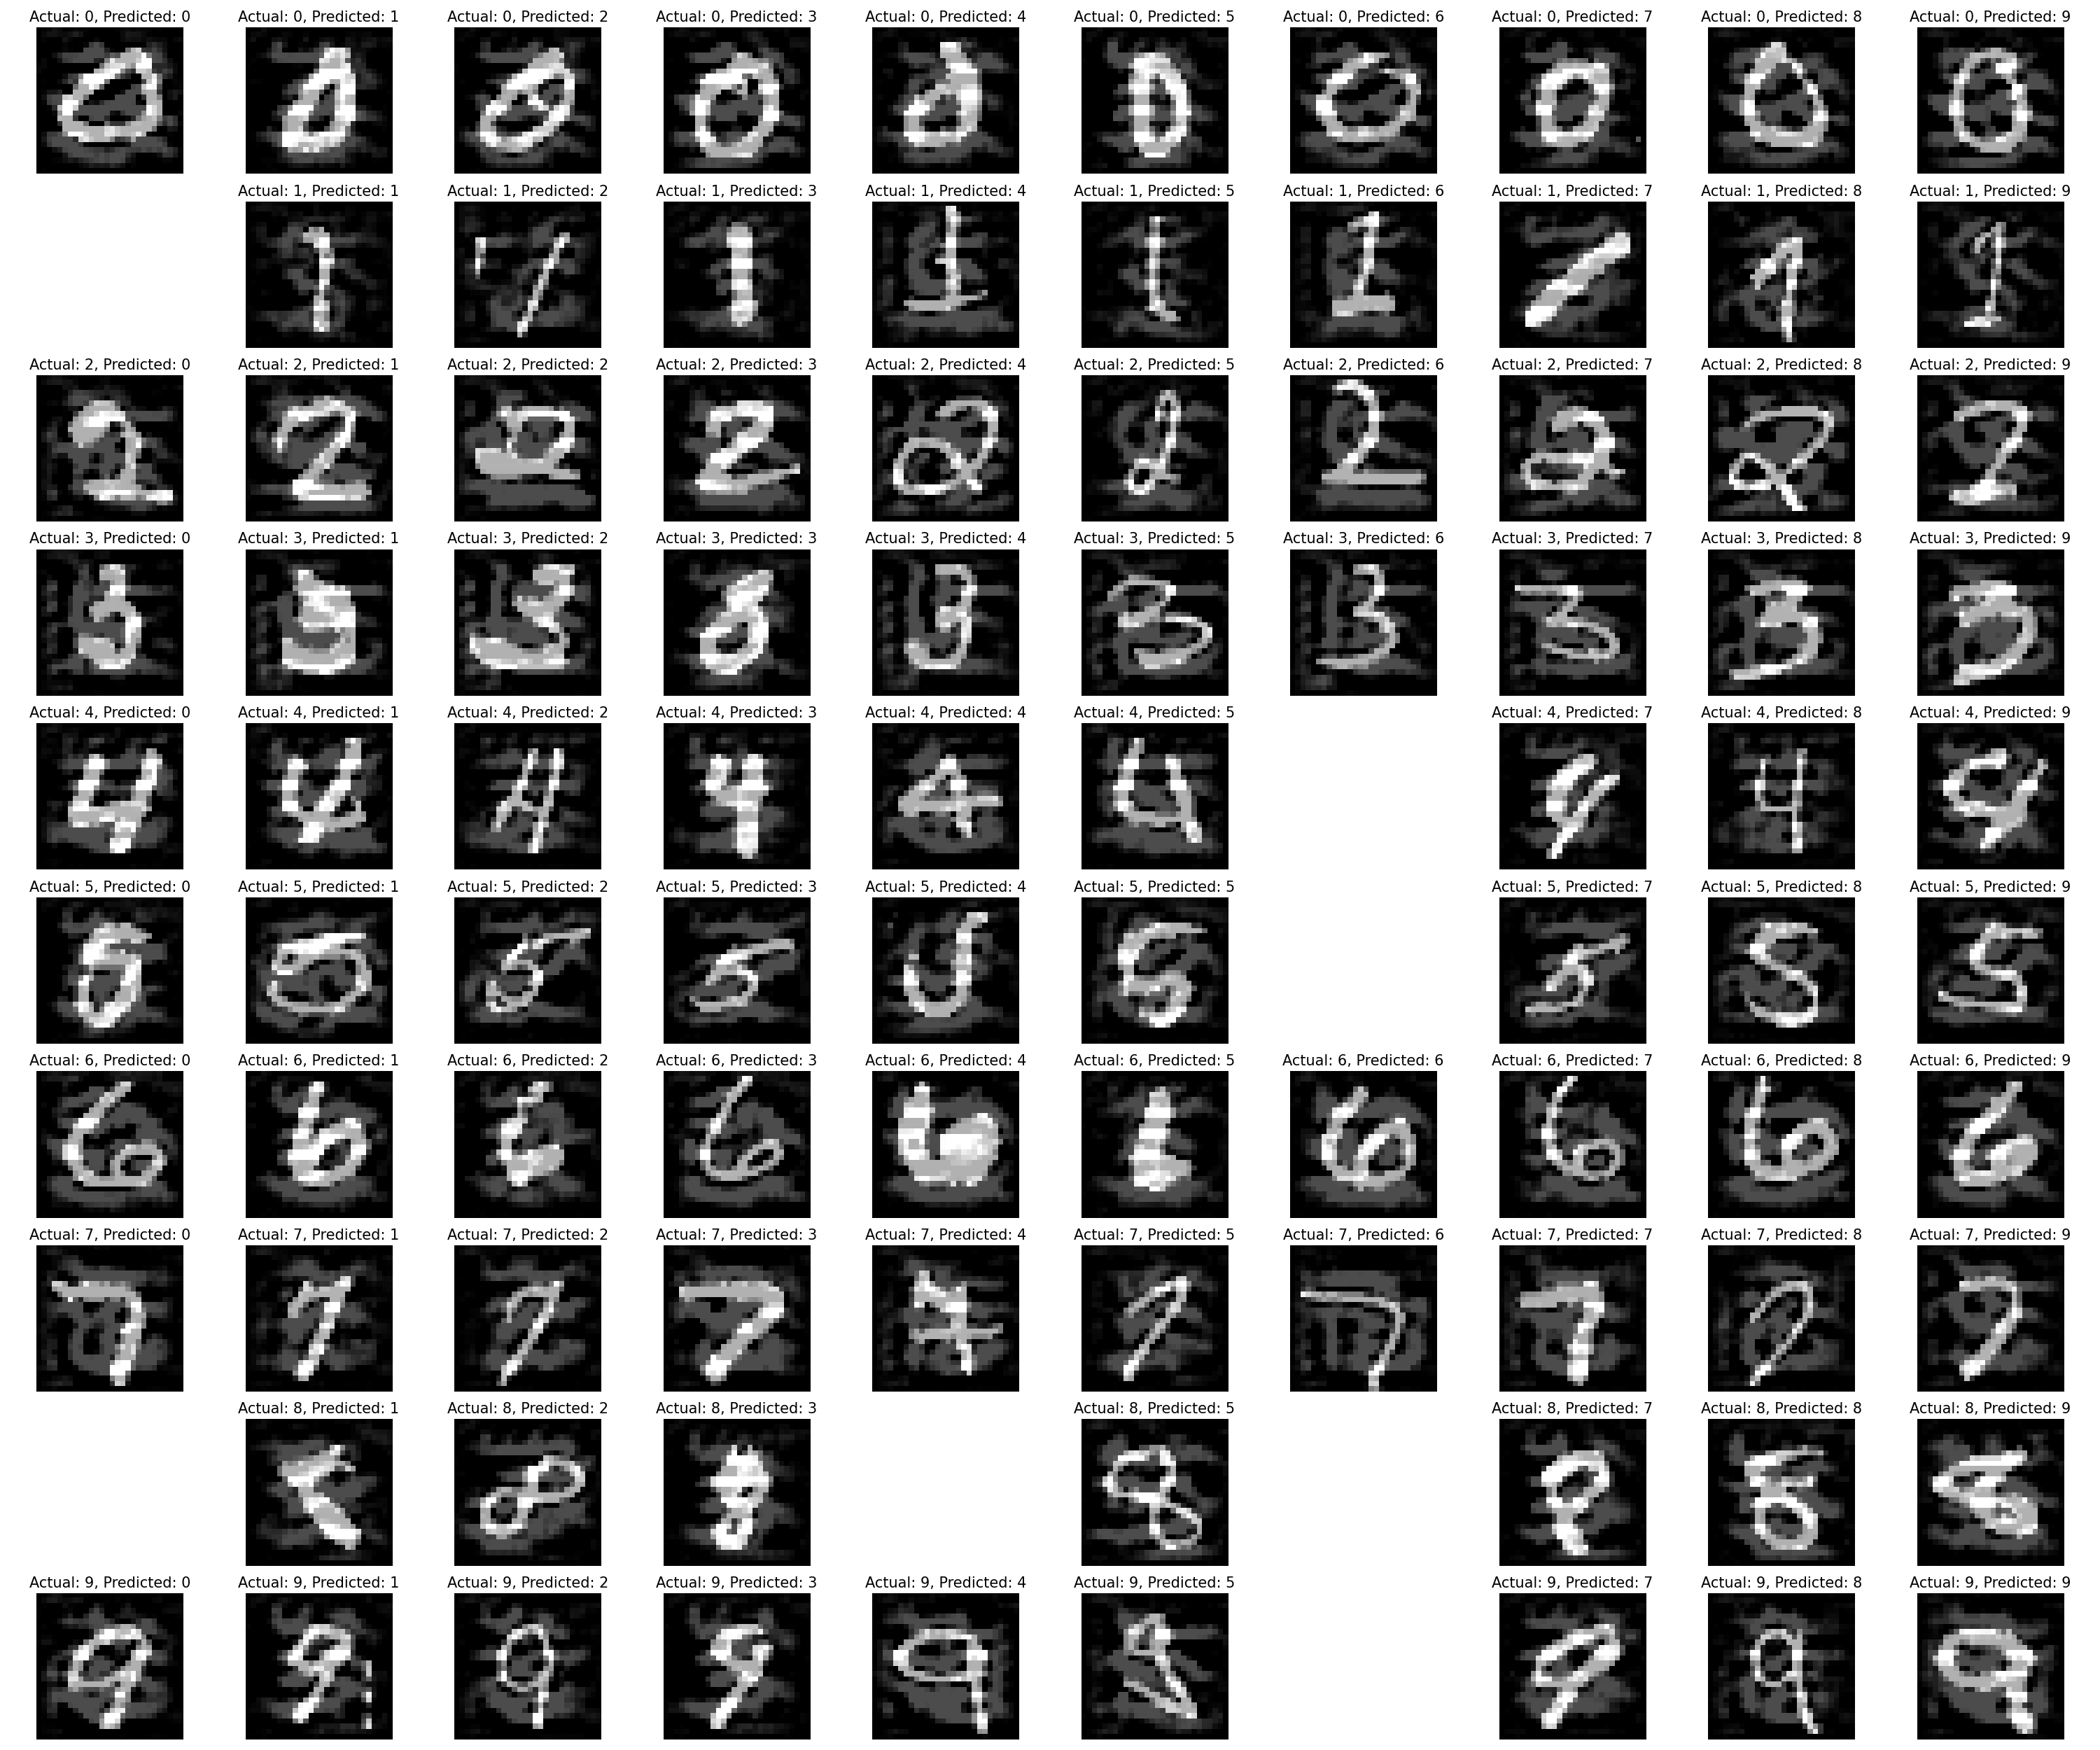
\includegraphics[width=\linewidth]{images/trainset_imgs_matrix.png}}
	\caption{نمونه‌های تقابلی تولید شده از تصویر‌های داده 
		\textbf{آموزش}
		 به همراه کلاس اصلی و کلاس پیش‌بینی شده}
	\label{trainset_imgs_matrix}
\end{figure}

\begin{figure}[H]
	\center{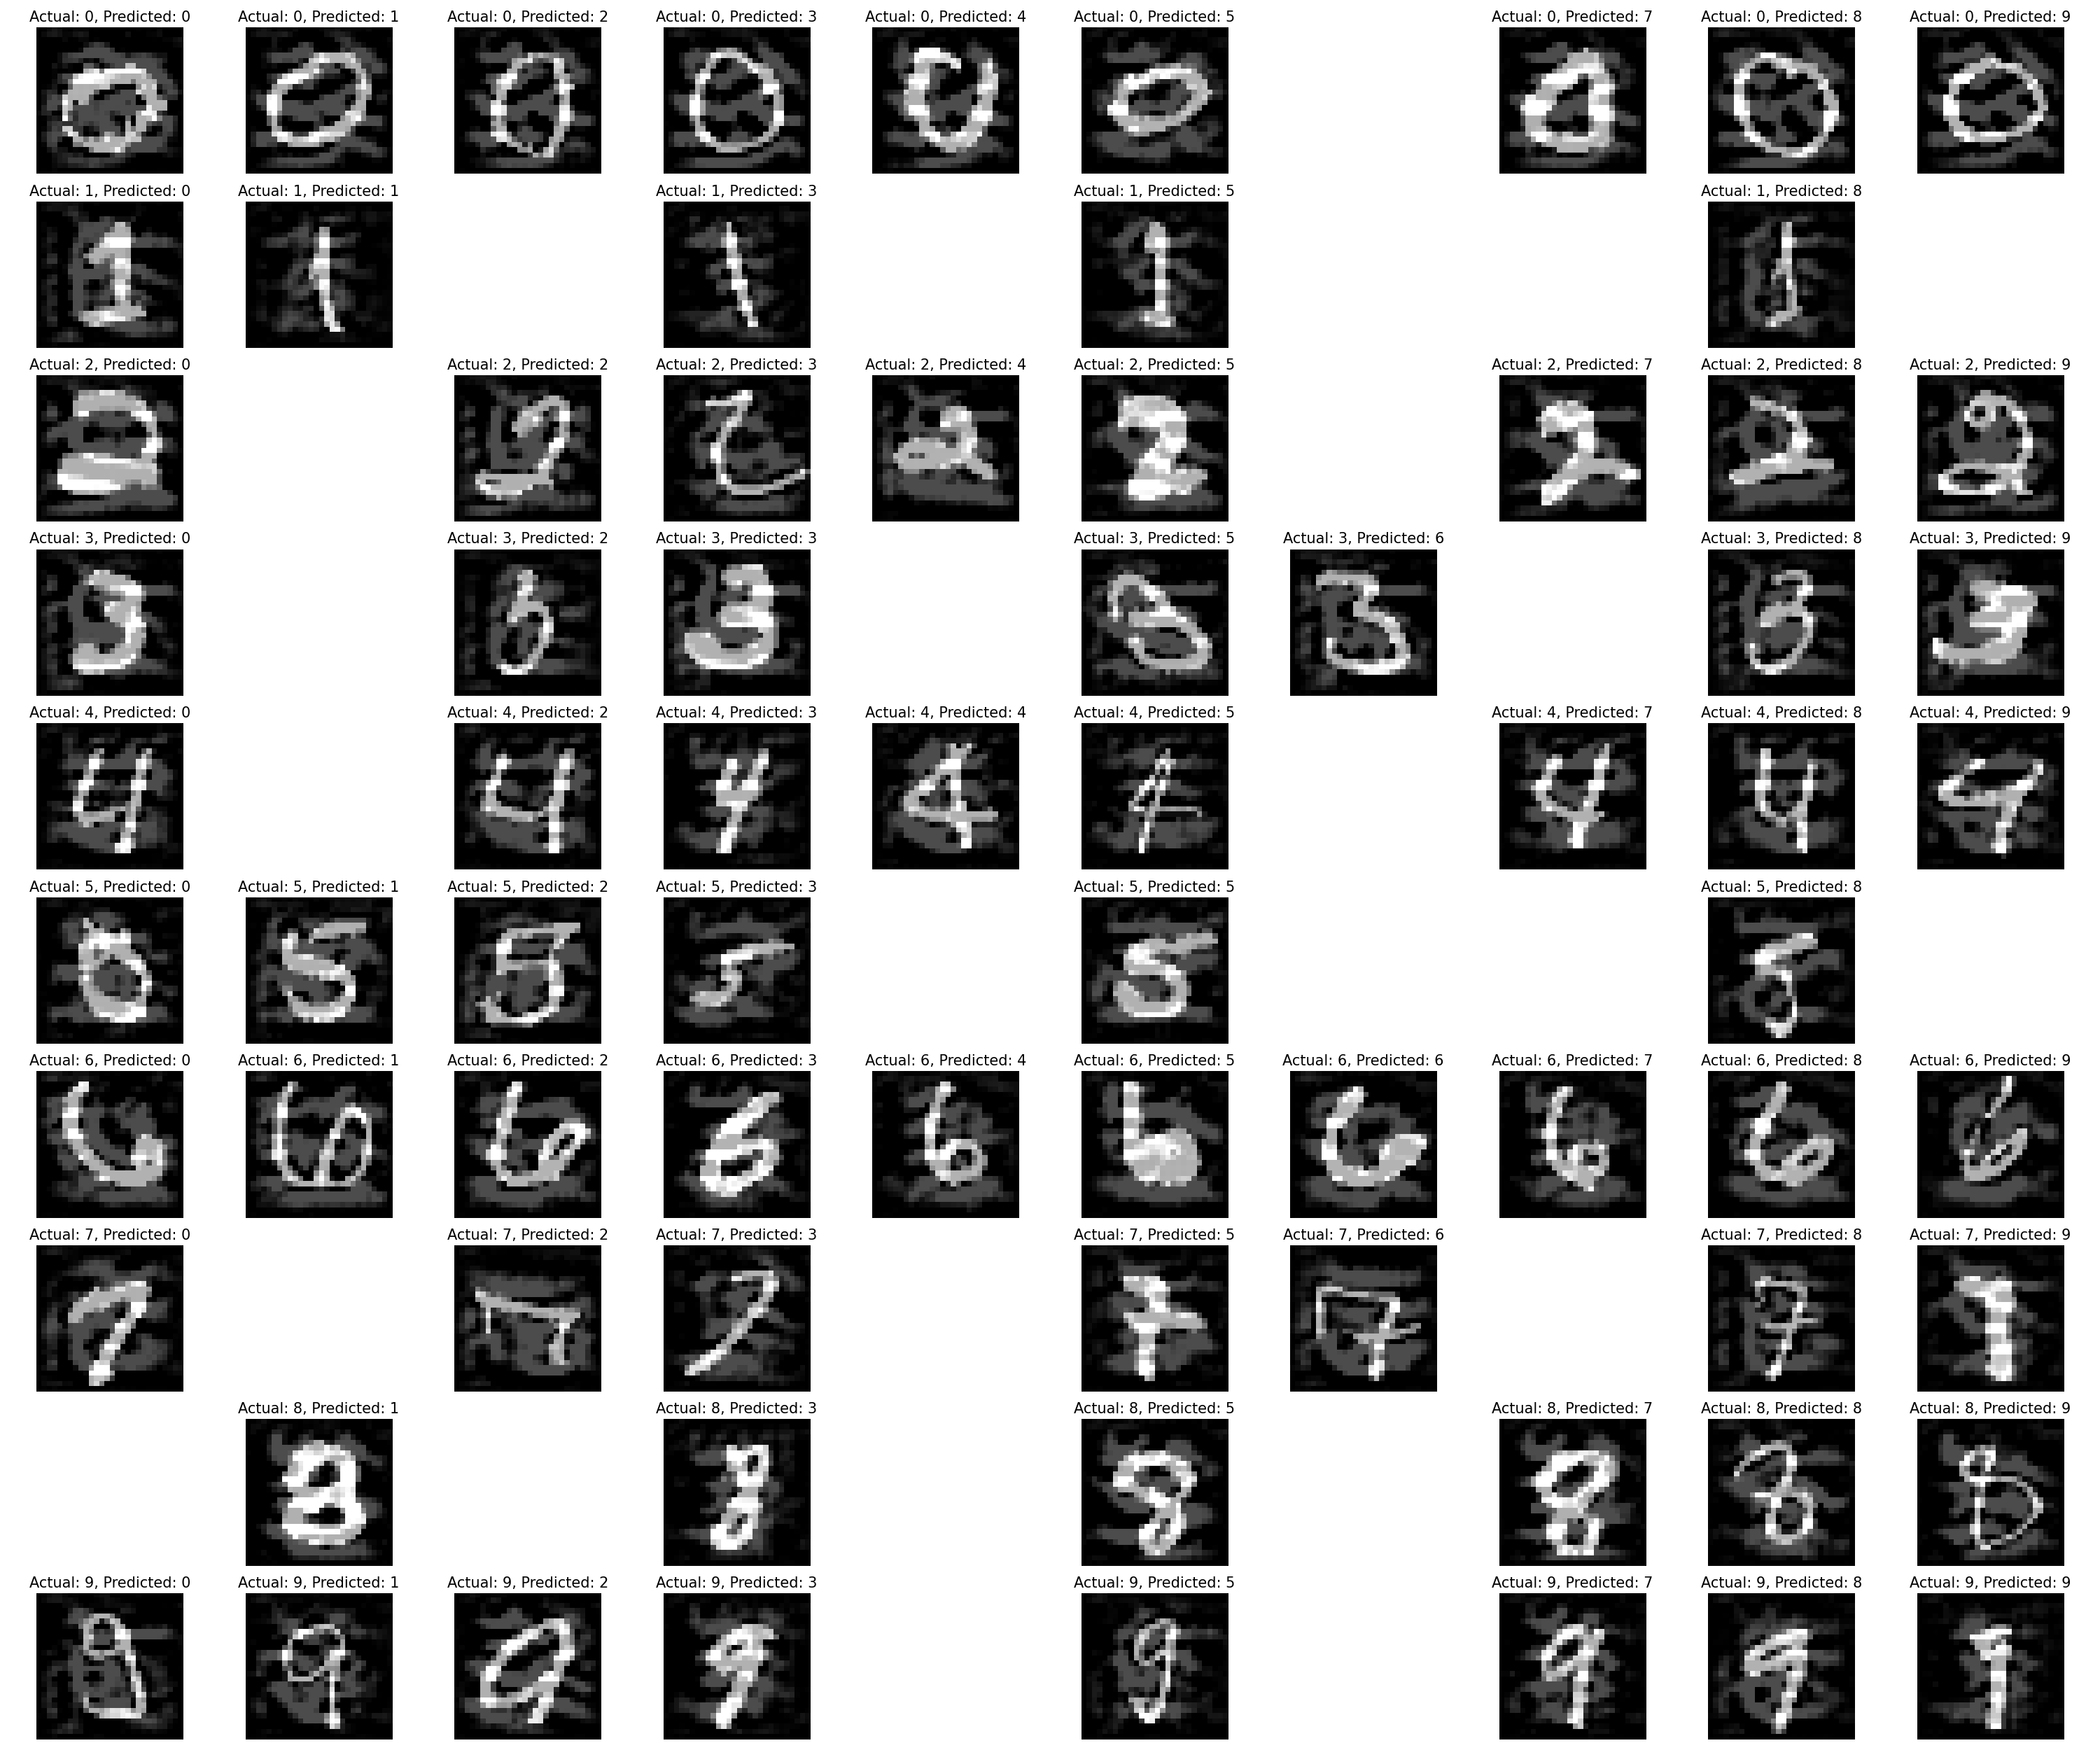
\includegraphics[width=\linewidth]{images/testset_imgs_matrix.png}}
	\caption{نمونه‌های تقابلی تولید شده از تصویر‌های داده
		 \textbf{تست} 
		به همراه کلاس اصلی و کلاس پیش‌بینی شده}
	\label{testset_imgs_matrix}
\end{figure}
لازم به ذکر است که در شکل‌های
\ref{trainset_imgs_matrix} 
و 
\ref{testset_imgs_matrix} 
جاهای خالی به این علت وجود دارند که ممکن است مدل هدف هنگامی که یک تصویر با برچسب اصلی ۰ به آن داده می‌شود را هیچ‌گاه شبیه به دسته‌ی ۶ طبقه بندی نکند و از این رو نمونه‌ی تقابلی‌ای برای این حالت در شکل وجود ندارد.

\newpage
در شکل‌های
\ref{trainset_confusion_matrix} 
و 
\ref{testset_confusion_matrix} 
نیز ماتریس درهم‌ریختگی برای نمونه‌های تقابلی بدست آمده از داده‌های آموزش و تست آورده شده است. در این ماتریس ردیف‌هانشان دهنده برچسب اصلی و ستون‌ها نشان دهنده‌ی برچسب پیش‌بینی شده توسط مدل هدف هستند.
\\
قطر ماتریس نشان‌دهنده تعداد پیش‌بینی‌های صحیح برای هر برچسب و دسته (برچسب پیش‌بینی شده با برچسب اصلی یکسان است) است. همان طور که ملاحظه می‌شود بیشتر نمو‌نه‌های تقابلی در دسته‌ای به غیر از دسته درست خود قرار گرفتند. همچنین مشاهده می‌شود که به طور مثال بیشتر نمونه‌های تقابلی‌ای که از تصویر‌های کلاس ۱ آموزشی تولید شده‌اند، از نظر شبکه هدف بیشتر به کلاس ۳ شباهت داشته‌اند.
\begin{figure}[H]
	\center{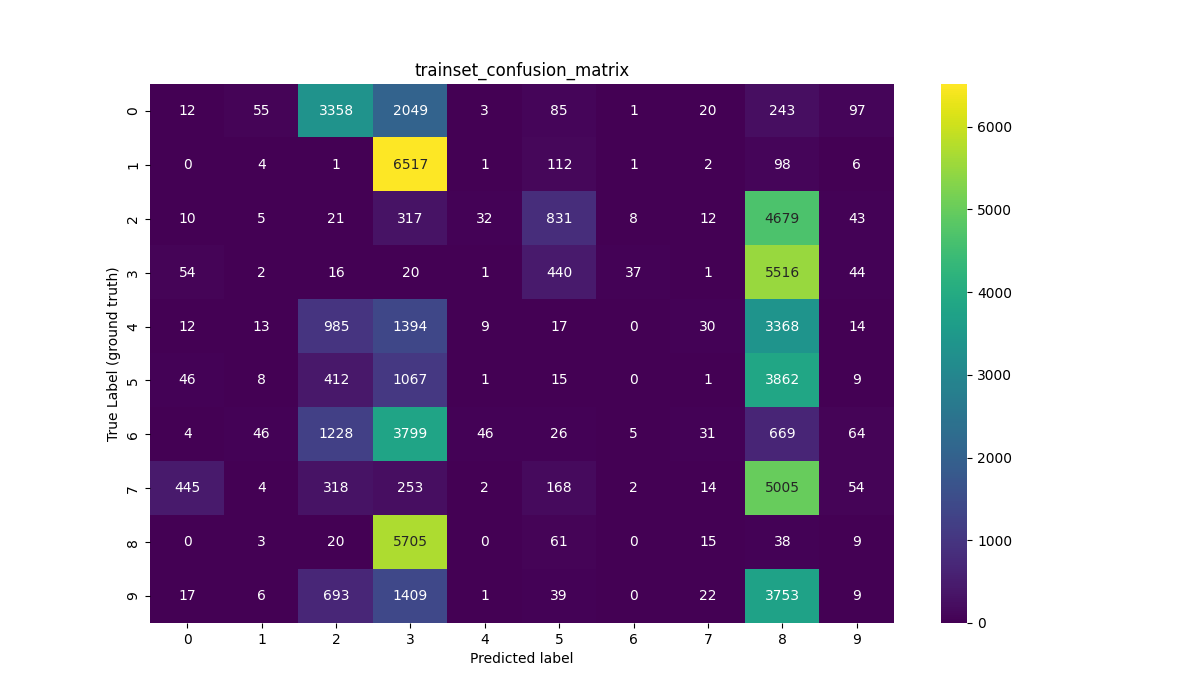
\includegraphics[width=\linewidth]{images/trainset_confusion_matrix.png}}
	\caption{ماتریس درهم‌ریختگی برای نمونه‌های تقابلی تولید شده از تصویر‌های داده آموزش}
	\label{trainset_confusion_matrix}
\end{figure}

\begin{figure}[H]
	\center{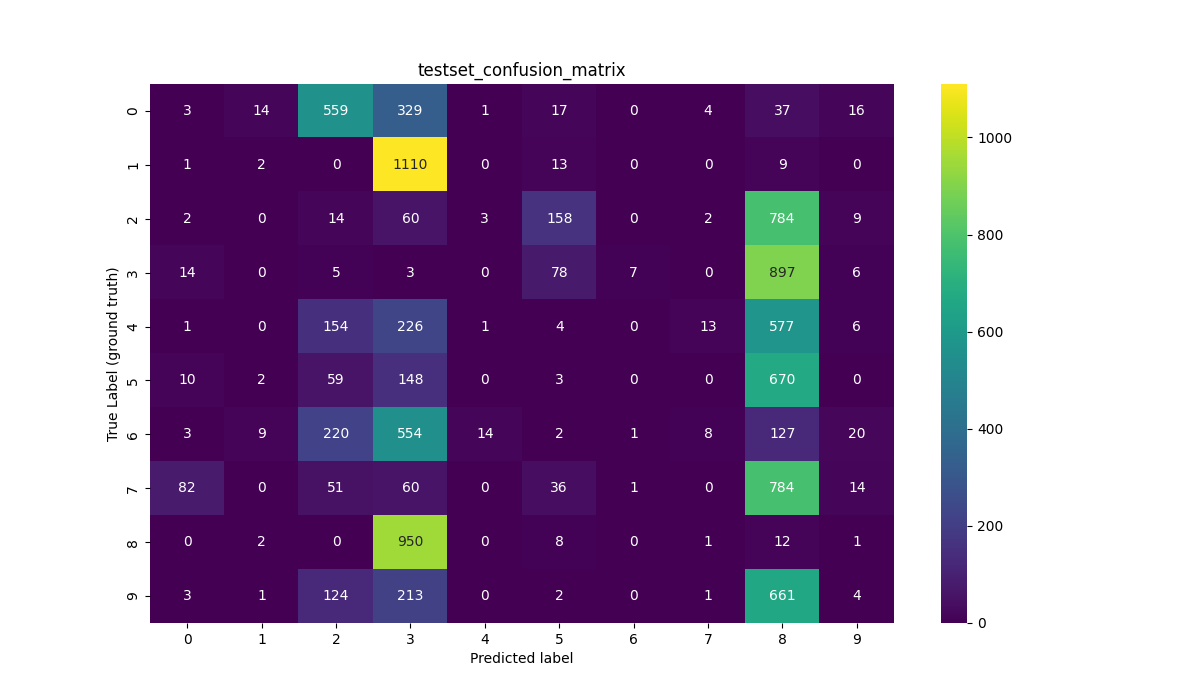
\includegraphics[width=\linewidth]{images/testset_confusion_matrix.png}}
	\caption{ماتریس درهم‌ریختگی برای نمونه‌های تقابلی تولید شده از تصویر‌های داده تست}
	\label{testset_confusion_matrix}
\end{figure}